%%%%%%%%%%%%%%%%%%%%%%%%%%%%%%%%%%%%%%%%%%%%%%%%%%%%%%%%
%%%%                                              %%%%%%
%%%%  Author: Peter Wilson                        %%%%%%
%%%%                                              %%%%%%
%%%%  ANDES quad element                          %%%%%%
%%%%                                              %%%%%%
%%%%%%%%%%%%%%%%%%%%%%%%%%%%%%%%%%%%%%%%%%%%%%%%%%%%%%%%


%fref generates automatically the respective abreviation/word in the text for the reference. You just have to define a label starting with the respective keyword.
%english: chap, sec, fig, eq, app
%deutsch: chap/kap, abs, abb, gl, anh
%see http://ctan.space-pro.be/tex-archive/macros/latex/contrib/fancyref/fancyref.pdf for more information



\setcounter{MaxMatrixCols}{20}
%\captionsetup{justification=centering}


\chapter{A brief background of shell elements}

As discussed in the introduction, shell elements are composed of membrane and bending contributions. The membrane contribution describes the behaviour of the x and y translational and the z rotational $(u_{x},\ u_{y},\ \theta_{z})$ degree of freedoms (DOFs) for each node, while the bending contribution is responsible for the z translational and x and y rotational $(u_{z},\ \theta_{x},\ \theta_{y})$ DOFs for each node.

\begin{figure}[H]
	\centering
	\def\svgwidth{\columnwidth}
	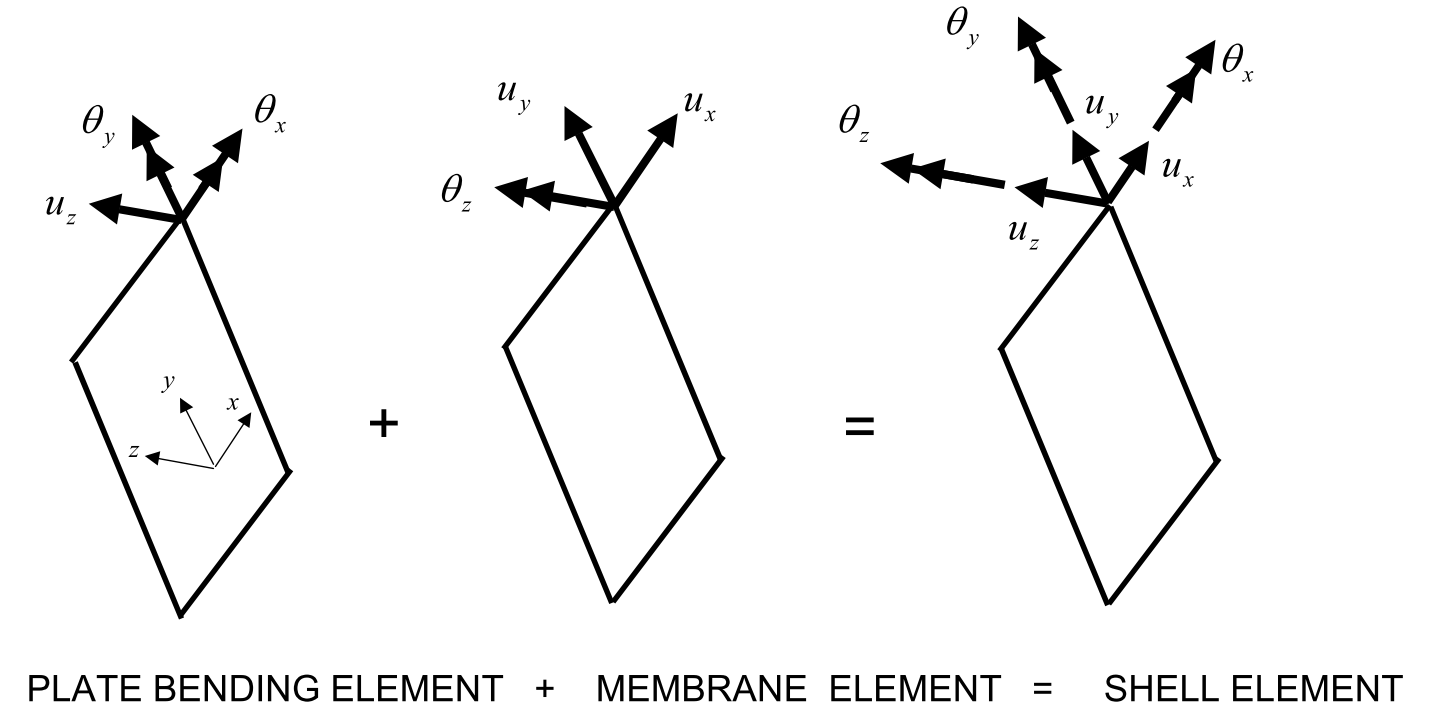
\includegraphics[width=12cm]{images/bendplusmemequalshell.png}
	\caption{Construction of shell DOFs from bending and membrane DOFs \\ (source: http://www.edwilson.org/BOOK-Wilson/10-SHE~1.pdf)}
	\label{bendplusmemequalshell}
\end{figure}

Furthermore, shells themselves are commonly divided into two groups, thin shells and thick shells, based on the underlying physics assumptions and kinematics. \\

Thin shells, governed by Kirchhoff bending plate theory, are analogous to Bernoulli beam elements where the shell directors remain straight and normal to the shell midsurface. This kinematic prescription neglects the transverse shear strains $\gamma_{xz}$ and $\gamma_{yz}$ as per the figure below.

\begin{figure}[H]
	\centering
	\def\svgwidth{\columnwidth}
	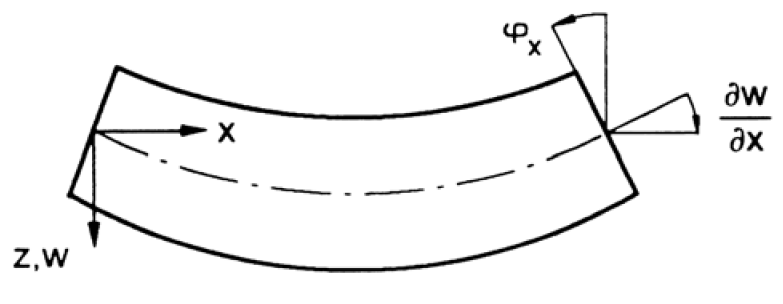
\includegraphics[width=6cm]{images/bernoullie.png}
	\caption{Thin (Kirchhoff) shell kinematics \\ (source: KU Bletzinger - Theory of Plates Lecture, 2016, TUM)}
	\label{thinshellkine}
\end{figure}

Contrasting this, thick shells adhering to Reissner Mindlin bending plate theory are analogous to Timoshenko beam elements, in that they consider the transverse shear deformations neglected by thin shells. The following figure highlights the kinematics of thick shells.

\begin{figure}[H]
	\centering
	\def\svgwidth{\columnwidth}
	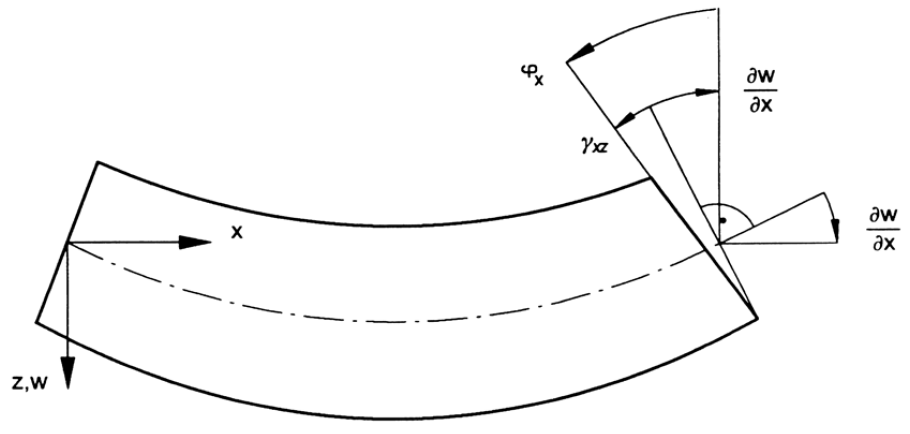
\includegraphics[width=10cm]{images/reissner.png}
	\caption{Thick (Reissner Mindlin) shell kinematics \\ (source: KU Bletzinger - Theory of Plates Lecture, 2016, TUM)}
	\label{thickshellkine}
\end{figure}

This work considers the implementation of a thin (Kirchhoff bending theory) quadrilateral shell element.

\subsection{Formulation context}

The context in which the following derivation operates within is hereby established. A general form of the linear static FEM is presented below.

\begin{equation} 
\textbf{K} \textbf{u} = \textbf{f}
\label{equation01}
\end{equation}

Since the proposed element is to be integrated into the existing multiphysics code KRATOS, the relevant term for the derivation of a new element is the system stiffness matrix $\textbf{K}$, which is constructed as such:

\begin{equation} 
\textbf{K} = \textbf{B}^T \textbf{C} \textbf{B} 
\label{equation02}
\end{equation}

$\textbf{C}$ is the constitutive matrix containing the material properties and physics, formed from the membrane and bending constitutive matrices. For the thin quad only a homogeneous isotropic plate constitutive law \cite{Bat82} is considered, as described below.

\begin{equation} 
\textbf{C} = 
\begin{pmatrix}
\frac{E}{(1-\nu^2)}
\begin{pmatrix}
1 & \nu & 0 \\
\nu & 1 & 0 \\
0 & 0 & (1-\nu)/2
\end{pmatrix}
& \mathbf{0} \\

\mathbf{0} & \frac{E t^3}{12(1-\nu^2)}
\begin{pmatrix}
1 & \nu & 0 \\
\nu & 1 & 0 \\
0 & 0 & (1-\nu)/2
\end{pmatrix}
\end{pmatrix}
\label{equation03}
\end{equation}

Thus, it is evident that the bulk of the element derivation lies in the determination of the element's strain displacement matrix $\textbf{B}$. The shell B matrix is composed of a membrane part and a bending part.






\chapter{ANDES-DKT quadrilateral shell element}

The formulation of the stiffness matrix for the thin quadrilateral shell element is presented after a quick orientation.

\section{Stiffness matrix}

asdfasdf



\subsection{Membrane formulation}

The membrane formulation is responsible for providing the membrane stiffness of the element. The membrane formulation chosen was the Assumed Natural Deviatoric Strains (ANDES) formulation as presented in \cite{Hau94}. A full description and theoretical derivation of the ANDES approach falls outside the scope of this document, however, those interested are directed to Militello's and Felippa's initial paper \cite{Fel91} on the formulation. Most importantly, the ANDES approach yields high performance elements that are insensitive to distortion.\\

Only the membrane portion of the total shell element is considered in this section, in which there are three DOFs per node.

\begin{equation} 
\mathbf{u^T} = 
\begin{pmatrix}
\mathbf{u_1} & \mathbf{u_2} & \mathbf{u_3} & \mathbf{u_4}
\end{pmatrix} 
\hspace{10mm}
where
\hspace{10mm}
\mathbf{u{_i}^T} = 
\begin{pmatrix}
{u_{xi}} & {u_{yi}} & {\theta_{zi}}
\end{pmatrix}
\label{equation04}
\end{equation}

The ANDES membrane formulation itself is split into the basic stiffness and the higher order stiffness.

\begin{equation} 
\mathbf{K}_{mem} = \mathbf{K}_{b} + \mathbf{K}_{h} = \int_A (\mathbf{L} + \mathbf{B}_h)^T \mathbf{C}_{mem} (\mathbf{L} + \mathbf{B}_h)\ dA
\label{equationMEM}
\end{equation}

The basic strain displacement matrix $\textbf{L}$ and the higher order complement $\textbf{B}_h$ are now developed. 

\subsubsection{Membrane basic stiffness}

The membrane basic stiffness is driven by assuming a constant stress field within the element and lumping this over side edges to consistent nodal forces. 

\begin{equation} 
\mathbf{f} = \boldsymbol{L\sigma}
\hspace{10mm}
where
\hspace{10mm}
\boldsymbol{\sigma^T} =
\begin{pmatrix}
\sigma_{xx} & \sigma_{xx} & \tau_{xy}
\end{pmatrix}
\label{equation05}
\end{equation}

The structure of the above expression is resolved as such: 

\begin{equation} 
\mathbf{L} =
\begin{pmatrix}
\mathbf{L_1} & \mathbf{L_2} & \mathbf{L_3} & \mathbf{L_4}
\end{pmatrix}
\hspace{10mm}
and
\hspace{10mm}
\mathbf{f} =
\begin{pmatrix}
\mathbf{f_1} \\
\mathbf{f_2} \\
\mathbf{f_3} \\
\mathbf{f_4}
\end{pmatrix}
\hspace{10mm}
where
\hspace{10mm}
\mathbf{f_i} =
\begin{pmatrix}
{f_{xi}} \\
{f_{yi}} \\
{m_{zi}}
\end{pmatrix}
\label{equation06}
\end{equation}

where each nodal entry '$j$' of the lumping matrix $\textbf{L}$ is constructed with the following cyclic permutation $(i,\ j,\ k,\ l)$ for the four nodes $(1,\ 2,\ 3,\ 4)$:

\begin{equation} 
\mathbf{L_j} = \frac{1}{2 A}
\begin{pmatrix}
y_{ki} & 0 & -x_{ki} \\
0 & -x_{ki} & y_{ki} \\
\frac{\alpha}{6}(y_{ij}^2 - y_{kj}^2 ) & \frac{\alpha}{6}(x_{ij}^2 - x_{kj}^2 ) & \frac{\alpha}{3}(x_{kj}y_{kj} - x_{ij}y_{ij})
\end{pmatrix}
\label{equation07}
\end{equation}

Throughout this paper the notation of $x_{ij} = x_i - x_j$ and $y_{ij} = y_i\ -\ y_j$ holds. Furthermore, the value of $\alpha$ is taken as 1.5 \cite{Fel91}.

\subsubsection{Membrane higher order stiffness}

The membrane higher order stiffness considers a set of higher order DOFs expressed in terms of the visible DOFs as per equation \eqref{equation04}.\\

\textit{It should be noted that the derviation below slightly departs from the formulation of Haugen \cite{Hau94} due to the DOF ordering as per equation \eqref{equation04}.}\\

The higher order rotational DOFs are related to the visible DOFs as described below:

\begin{equation} 
\boldsymbol{\theta_h} = \mathbf{H_{\theta v}} \mathbf{u}
\hspace{10mm}
where
\hspace{10mm}
\boldsymbol{\theta_{h}^T} = 
\begin{pmatrix}
\theta_1^{'} & \theta_2^{'} & \theta_3^{'} & \theta_4^{'} & \bar{\theta}
\end{pmatrix}
\label{equation08}
\end{equation}

with

\begin{gather} 
	\begin{aligned}
		&\mathbf{H_{\theta v}} = 
		\begin{pmatrix}
			0 & 0 & \frac{3}{4} & 0 & 0 & \frac{-1}{4} & 0 & 0 & \frac{-1}{4} & 0 & 0 & \frac{-1}{4} \\
			0 & 0 & \frac{-1}{4} & 0 & 0 & \frac{3}{4} & 0 & 0 & \frac{-1}{4} & 0 & 0 & \frac{-1}{4} \\
			0 & 0 & \frac{-1}{4} & 0 & 0 & \frac{-1}{4} & 0 & 0 & \frac{3}{4} & 0 & 0 & \frac{-1}{4} \\
			0 & 0 & \frac{-1}{4} & 0 & 0 & \frac{-1}{4} & 0 & 0 & \frac{-1}{4} & 0 & 0 & \frac{3}{4} \\
			\frac{x_{42}}{f} & \frac{y_{42}}{f} & \frac{1}{4} & \frac{x_{13}}{f} & \frac{y_{13}}{f} & \frac{1}{4} & \frac{x_{24}}{f} & \frac{y_{24}}{f} & \frac{1}{4} & \frac{x_{31}}{f} & \frac{y_{31}}{f} & \frac{1}{4}
		\end{pmatrix}\\
		&where 
		\hspace{10mm} 
		f = 16{|}\mathbf{J}{|}\\
		\hspace{10mm}
		&and
		\hspace{10mm}
		{|}\mathbf{J}{|} = \frac{1}{8}[ (x_1 y_2 - x_2 y_1) + (x_2 y_3 - x_3 y_2) + (x_3 y_4 - x_4 y_3) + (x_4 y_1 - x_1 y_4)]
		\label{equation09}
	\end{aligned}
\end{gather}

The higher order translational DOFs are related to the visible DOFs as described below:

\begin{equation} 
\widetilde{\mathbf{v}}_t = \mathbf{H}_{tv} \mathbf{u}
\hspace{10mm}
where
\hspace{10mm}
\widetilde{\mathbf{v}}_t^T = 
\begin{pmatrix}
\widetilde{v}_x & \widetilde{v}_y
\end{pmatrix}
\label{equationv_t}
\end{equation}

with

\begin{equation} 
\mathbf{H_{tv}} =
\begin{pmatrix}
1 & 0 & 0 & -1 & 0 & 0 & 1 & 0 & 0 & -1 & 0 & 0 \\
0 & 1 & 0 & 0 & -1 & 0 & 0 & 1 & 0 & 0 & -1 & 0 & 
\end{pmatrix}
\label{equation10}
\end{equation}

Combining both mapping matrices together expresses all higher order DOFs in terms of the visible DOFs:

\begin{equation} 
\widetilde{\mathbf{v}} = \mathbf{H v}
\hspace{10mm}
where
\hspace{10mm}
\mathbf{H} =
\begin{pmatrix}
\mathbf{H_{\theta v}} \\
\mathbf{H_{vt}}
\end{pmatrix}
\hspace{10mm}
and
\hspace{10mm}
\widetilde{\mathbf{v}}^T = 
\begin{pmatrix}
\theta_1^{'} & \theta_2^{'} & \theta_3^{'} & \theta_4^{'} & \bar{\theta} &  \widetilde{v}_x & \widetilde{v}_y
\end{pmatrix}
\label{equation11}
\end{equation}

The descriptions for equations from \eqref{equation12} to \eqref{equation22} are heavily abridged from the original element derivation \cite{Hau94}. The general idea of these equations is to relate the higher order nodal strain gauge readings to cartesian strain displacement matrices $\mathbf{B}_{hi}$.\\

The components necessary for the construction of the higher order bending strain field (along $\xi$ and $\eta$ directions) are shown below:

\begin{equation} 
\chi_{\xi | i} = \frac{d_{\xi | i}}{l_\xi},
\hspace{10mm}
\chi_{\eta | i} = \frac{d_{\eta | i}}{l_\eta},
\label{equation12}
\end{equation}

where

\begin{align*} 
	d_{\xi | i} = \sqrt{(\mathbf{r_i} \times \mathbf{s_\xi}) \cdot (\mathbf{r_i} \times \mathbf{s_\xi})}\ ,
	\hspace{10mm}
	l_\xi = \sqrt{\mathbf{r_\xi} \cdot \mathbf{r_\xi}}\ ,
	\hspace{10mm} 
	\mathbf{r_\xi} = \frac{1}{2} ( \mathbf{r_2} + \mathbf{r_3} - \mathbf{r_1} - \mathbf{r_4} )\ , \\
	d_{\eta | i} = \sqrt{(\mathbf{r_i} \times \mathbf{s_\eta}) \cdot (\mathbf{r_i} \times \mathbf{s_\eta})}\ ,
	\hspace{10mm}
	l_\xi = \sqrt{\mathbf{r_\eta} \cdot \mathbf{r_\eta}}\ ,
	\hspace{10mm}
	\mathbf{r_\eta} = \frac{1}{2} ( \mathbf{r_2} + \mathbf{r_3} - \mathbf{r_1} - \mathbf{r_4} )\ ,
\end{align*}


$\textbf{s}_\xi$ and $\textbf{s}_\eta$ are the normalized parametric base vectors in cartesian coordinates, while $\textbf{r}_i$ are the nodal position vectors in cartesian coordinates.\\

The components necessary for the construction of the higher order bending strain field (along the element diagonal) are shown below: 


\begin{equation} 
\chi_{24} = \frac{d_{24}}{2 l_{24}},
\hspace{10mm}
\chi_{13} = \frac{d_{13}}{2 l_{13}},
\label{equation12chi24}
\end{equation}

where

\begin{align*} 
	d_{24} = d_{13} = \sqrt{(\mathbf{r_{31}} \times \mathbf{e_{24}}) \cdot (\mathbf{r_{31}} \times \mathbf{e_{24}})} \\
	l_{24} = \sqrt{\mathbf{r_{24}} \cdot \mathbf{r_{24}}}\ ,
	\hspace{10mm}
	\mathbf{r_{24}} = \mathbf{r_2} - \mathbf{r_4} \\
	l_{13} = \sqrt{\mathbf{r_{13}} \cdot \mathbf{r_{13}}}\ ,
	\hspace{10mm}
	\mathbf{r_{13}} = \mathbf{r_1} - \mathbf{r_3}
	\hspace{10mm}
	\mathbf{e}_{24} = \frac{\mathbf{r}_{24}}{l_{24}}
\end{align*}

The components necessary for the construction of the higher order torsional strain field are shown below:

\begin{equation} 
\chi_{\xi t} = \frac{l_\eta}{l_\xi}\ ,
\hspace{10mm}
\chi_{\eta t} = \frac{l_\xi}{l_\eta}\ ,
\label{equation13}
\end{equation}


The mapping from strain gauge readings along the 3 directions at each node to the higher order DOFs is via the matrices $\mathbf{Q}_i$ described below:


\begin{equation} 
\mathbf{Q_1} =
\begin{pmatrix}
\rho_1 \chi_{\xi | 1} & \rho_2 \chi_{\xi | 1} & \rho_3 \chi_{\xi | 1} & \rho_4 \chi_{\xi | 1} & \alpha \chi_{\xi t} & -\beta_1 \frac{\chi_{\xi | 1}}{\bar{\chi_\xi} l_\xi} & 0  \\	
-\rho_1 \chi_{\eta | 1} & -\rho_4 \chi_{\eta | 1} & -\rho_3 \chi_{\eta | 1} & -\rho_2 \chi_{\eta | 1} & -\alpha \chi_{\eta t} & 0 & -\beta_1 \frac{\chi_{\eta | 1}}{\bar{\chi_\eta} l_\eta} \\
\rho_5 \chi_{24} & \rho_6 \chi_{24} & \rho_7 \chi_{24} & \rho_8 \chi_{24} & 0 & \beta_2 \frac{c_{24 \xi}}{l_{24}} & -\beta_2 \frac{c_{24 \eta}}{l_{24}}
\end{pmatrix}		
\label{equation14}
\end{equation}

\begin{equation} 
\mathbf{Q_2} =
\begin{pmatrix}
-\rho_2 \chi_{\xi | 2} & -\rho_1 \chi_{\xi | 2} & -\rho_4 \chi_{\xi | 2} & -\rho_3 \chi_{\xi | 2} & -\alpha \chi_{\xi t} & -\beta_1 \frac{\chi_{\xi | 2}}{\bar{\chi_\xi} l_\xi} & 0  \\	
\rho_4 \chi_{\eta | 2} & \rho_1 \chi_{\eta | 2} & \rho_2 \chi_{\eta | 2} & \rho_3 \chi_{\eta | 2} & \alpha \chi_{\eta t} & 0 & \beta_1 \frac{\chi_{\eta | 2}}{\bar{\chi_\eta} l_\eta} \\
\rho_8 \chi_{13} & \rho_5 \chi_{13} & \rho_6 \chi_{13} & \rho_7 \chi_{13} & 0 & -\beta_2 \frac{c_{13 \xi}}{l_{13}} & \beta_2 \frac{c_{13 \eta}}{l_{13}}
\end{pmatrix}		
\label{equation14_2}
\end{equation}

\begin{equation} 
\mathbf{Q_3} =
\begin{pmatrix}
\rho_3 \chi_{\xi | 3} & \rho_4 \chi_{\xi | 3} & \rho_1 \chi_{\xi | 3} & \rho_2 \chi_{\xi | 3} & \alpha \chi_{\xi t} & \beta_1 \frac{\chi_{\xi | 3}}{\bar{\chi_\xi} l_\xi} & 0  \\	
-\rho_3 \chi_{\eta | 3} & -\rho_2 \chi_{\eta | 3} & -\rho_1 \chi_{\eta | 3} & -\rho_4 \chi_{\eta | 3} & -\alpha \chi_{\eta t} & 0 & \beta_1 \frac{\chi_{\eta | 3}}{\bar{\chi_\eta} l_\eta} \\
\rho_7 \chi_{13} & \rho_8 \chi_{13} & \rho_5 \chi_{13} & \rho_6 \chi_{213} & 0 & -\beta_2 \frac{c_{13 \xi}}{l_{13}} & \beta_2 \frac{c_{13 \eta}}{l_{13}}
\end{pmatrix}		
\label{equation14_3}
\end{equation}

\begin{equation} 
\mathbf{Q_4} =
\begin{pmatrix}
-\rho_4 \chi_{\xi | 4} & -\rho_3 \chi_{\xi | 4} & -\rho_2 \chi_{\xi | 4} & -\rho_1 \chi_{\xi | 4} & -\alpha \chi_{\xi t} & \beta_1 \frac{\chi_{\xi | 4}}{\bar{\chi_\xi} l_\xi} & 0  \\	
\rho_2 \chi_{\eta | 4} & \rho_3 \chi_{\eta | 4} & \rho_4 \chi_{\eta | 4} & \rho_1 \chi_{\eta | 4} & \alpha \chi_{\eta t} & 0 & -\beta_1 \frac{\chi_{\eta | 4}}{\bar{\chi_\eta} l_\eta} \\
\rho_6 \chi_{13} & \rho_7 \chi_{13} & \rho_8 \chi_{13} & \rho_5 \chi_{13} & 0 & \beta_2 \frac{c_{13 \xi}}{l_{13}} & -\beta_2 \frac{c_{13 \eta}}{l_{13}}
\end{pmatrix}		
\label{equation15}
\end{equation}

where

\begin{align*} 
	c_{13 \xi} = \mathbf{s_{13}^T} \mathbf{s_\xi}\ ,
	\hspace{10mm}
	c_{13 \eta} = \mathbf{s_{13}^T} \mathbf{s_\eta}\ ,
	\hspace{10mm}
	c_{24 \xi} = \mathbf{s_{24}^T} \mathbf{s_\xi}\ ,
	\hspace{10mm}
	c_{24 \eta} = \mathbf{s_{24}^T} \mathbf{s_\eta}
	\hspace{10mm}
\end{align*}

Values for the coefficients utilised above are as follows:

\begin{gather} 
	\begin{aligned}
		&\rho_1 = 0.1\ ,
		\hspace{10mm}
		\rho_2 = -0.1\ ,
		\hspace{10mm}
		\rho_3 = -0.1\ ,
		\hspace{10mm}
		\rho_4 = 0.1\ ,
		\hspace{10mm}
		\rho_5 = 0.0\ , \\
		&\rho_6 = 0.5\ ,
		\hspace{10mm}
		\rho_7 = 0.0\ ,
		\hspace{10mm}
		\rho_8 = -0.5\ ,
		\hspace{10mm}
		\beta_1 = 0.6\ ,
		\hspace{10mm}
		\beta_2 = 0.0
		\label{equation16}
	\end{aligned}
\end{gather}


The cartesian strain displacement matrices at the nodes are related to the mapping matrices $\mathbf{Q}_i$ as described below:


\begin{gather} 
	\begin{aligned}
		&\mathbf{B_{h1}} = \mathbf{T_{13}}  \mathbf{Q_{1}}\ ,
		\hspace{10mm}
		\mathbf{B_{h3}} = \mathbf{T_{13}}  \mathbf{Q_{3}}\\
		&where 
		\hspace{10mm} 
		\mathbf{T_{13}^{-1}} =
		\begin{pmatrix}
			s_{\xi x}^2 & s_{\xi y}^2 & s_{\xi x} s_{\xi y} \\
			s_{\eta x}^2 & s_{\eta y}^2 & s_{\eta x} s_{\eta y} \\
			s_{24 x}^2 & s_{24 y}^2 & s_{24 x} s_{24 y}
		\end{pmatrix}
		\label{equation17}
	\end{aligned}
\end{gather}


\begin{gather} 
	\begin{aligned}
		&\mathbf{B_{h2}} = \mathbf{T_{24}}  \mathbf{Q_{2}}\ ,
		\hspace{10mm}
		\mathbf{B_{h4}} = \mathbf{T_{24}}  \mathbf{Q_{4}}\\
		&where 
		\hspace{10mm} 
		\mathbf{T_{24}^{-1}} =
		\begin{pmatrix}
			s_{\xi x}^2 & s_{\xi y}^2 & s_{\xi x} s_{\xi y} \\
			s_{\eta x}^2 & s_{\eta y}^2 & s_{\eta x} s_{\eta y} \\
			s_{13 x}^2 & s_{13 y}^2 & s_{13 x} s_{13 y}
		\end{pmatrix}
		\label{equation18}
	\end{aligned}
\end{gather}

The higher order membrane B matrix $\mathbf{B}_h$ is constructed from the interpolation of the nodal B matrices with standard bi-linear shape functions.

\begin{equation} 
\mathbf{B_h}(\xi,\eta) = (1-\xi)(1-\eta)\mathbf{B_{h1}} + (1+\xi)(1-\eta)\mathbf{B_{h2}} + (1+\xi)(1+\eta)\mathbf{B_{h3}} +	(1-\xi)(1+\eta)\mathbf{B_{h4}} 
\label{equation19}
\end{equation}


\subsection{Bending formulation}

The bending formulation is responsible for providing the bending stiffness of the element. The bending formulation chosen was the Discrete Kirchhoff Quadrilateral (DKQ) formulation  originally presented by Batoz \cite{Bat82}, presented in a most readable fashion in the PhD dissertation of Barrales \cite{Bar12}. A full description and theoretical derivation of the DKQ approach falls outside the scope of this document, refer \cite{Bat82}. Most importantly for a thin shell element, the transverse shear strain energy is neglected which prohibits element performance deterioration as the ratio $\frac{l}{t}$ encroaches into thin and very thin plate territories.\\

Only the bending portion of the total shell element is considered in this section, in which there are three nodal DOFs per node $(w_i$ corresponds to $u_{zi}$ in the figure below).

\begin{figure}[H]
	\centering
	\def\svgwidth{\columnwidth}
	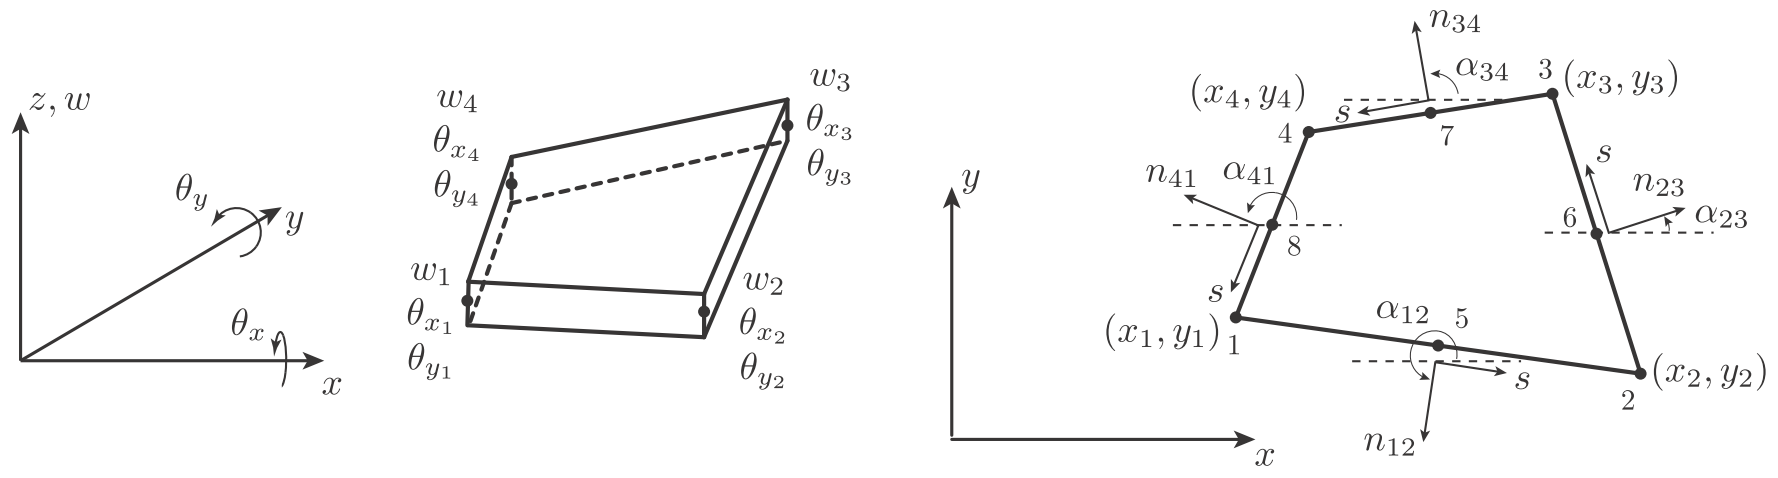
\includegraphics[width=15cm]{images/8nodeseren.png}
	\caption{DKQ DOF arrangement and geometry (source: \cite{Bar12})}
	\label{8nodeseren}
\end{figure}

\begin{equation} 
\mathbf{u^T} = 
\begin{pmatrix}
\mathbf{u_1} & \mathbf{u_2} & \mathbf{u_3} & \mathbf{u_4}
\end{pmatrix} 
\hspace{10mm}
where
\hspace{10mm}
\mathbf{u{_i}^T} = 
\begin{pmatrix}
{u_{zi}} & {\theta_{xi}} & {\theta_{yi}}
\end{pmatrix}
\label{equationBending}
\end{equation}

The nodal rotational interpolation employed is as per the 8 node serendipity quad element:

\begin{equation} 
\begin{pmatrix}
\beta_x (\xi , \eta) \\
\beta_y (\xi , \eta)
\end{pmatrix}
= \sum_{i=1}^8 \psi_i (\xi , \eta) 
\begin{pmatrix}
\beta_{xi} (\xi , \eta) \\
\beta_{yi} (\xi , \eta)
\end{pmatrix}
\label{equation20}
\end{equation}

where $\psi_i$ are the standard 8 node serendipity shape functions described by Zienkiewicz \cite{Zie77}:


\begin{gather} 
	\begin{aligned}
		&\psi_i (\xi , \eta) = \frac{-1}{4} (1 + \xi_i \xi)(1 + \eta_i \eta)(1 - \xi_i \xi - \eta_i \eta)
		\hspace{10mm}
		i = 1, 2, 3, 4 \\
		&\psi_i (\xi , \eta) = \frac{1}{2} (1 - \xi^2)(1 + \eta_i \eta)
		\hspace{10mm}
		i = 5, 7 \\
		&\psi_i (\xi , \eta) = \frac{1}{2} (1 + \xi_i \xi)(1 - \eta^2)
		\hspace{10mm}
		i = 6, 8
		\label{equation21}
	\end{aligned}
\end{gather}

and $\xi_i$ and $\eta_i$ are the natural coordinates of the 8 node serendipity element described in figure \ref{8nodeseren}.\\

The following derivation from equations \eqref{equation22} to \eqref{equation27} is heavily summarised from that of Barrales \cite{Bar12}. The general idea is the construction of a mapping from the standard 12 DOFs at each node to $\beta_x (\xi,\ \eta)$ and $\beta_y (\xi,\ \eta)$ across the element, the derivatives of which are curvatures as expressed in equation \eqref{equation27}.\\

The following quantities are required components for the mapping:

\begin{equation} 
L_{ij} = \sqrt{x_{ij}^2 + y_{ij}^2}\ ,
\hspace{10mm}
x_{ij} = x_i - x_j\ ,
\hspace{10mm}
y_{ij} = y_i - y_j
\label{equation22}
\end{equation}


\begin{gather} 
	\begin{aligned}
		&a_k = \frac{-x_{ij}}{L_{ij}^2}\ ,
		\hspace{10mm}
		b_k = \frac{3}{4} \frac{x_{ij} y_{ij}}{L_{ij}^2}\ , \\
		&c_k = \frac{\frac{1}{4} x_{ij}^2 - \frac{1}{2} y_{ij}^2}{L_{ij}^2}\ ,
		\hspace{10mm}
		d_k = \frac{-y_{ij}}{L_{ij}^2}\ ,
		\hspace{10mm}
		e_k = \frac{\frac{-1}{2} x_{ij}^2 + \frac{1}{4} y_{ij}^2}{L_{ij}^2}
		\label{equation23}
	\end{aligned}
\end{gather}

The elements of the mapping matrix are arranged as such:

\begin{equation} 
\mathbf{\Psi^x} = 
\begin{pmatrix}
\Psi_1^x \\
\vdots \\
\Psi_{12}^x
\end{pmatrix}\ ,
\hspace{10mm}
\mathbf{\Psi^y} = 
\begin{pmatrix}
\Psi_1^y \\
\vdots \\
\Psi_{12}^y
\end{pmatrix}
\label{equation24}
\end{equation}

where the vectors entries are calculated as per the following scheme:

\begin{gather} 
	\begin{aligned}
		&\Psi_{3(i-1)+1}^x (\xi , \eta) = \frac{3}{2} (a_r \psi_r (\xi , \eta) - a_s \psi_s (\xi , \eta) ) \\
		&\Psi_{3(i-1)+2}^x (\xi , \eta) = b_r \psi_r (\xi , \eta) + b_s \psi_s (\xi , \eta) \\
		&\Psi_{3(i-1)+3}^x (\xi , \eta) = \psi_i (\xi , \eta) - c_r \psi_r (\xi , \eta) - c_s \psi_s (\xi , \eta)
		\label{equation25}
	\end{aligned}
\end{gather}

\begin{gather} 
	\begin{aligned}
		&\Psi_{3(i-1)+1}^y (\xi , \eta) = \frac{3}{2} (d_r \psi_r (\xi , \eta) - d_s \psi_s (\xi , \eta) ) \\
		&\Psi_{3(i-1)+2}^y (\xi , \eta) = -\psi_i (\xi , \eta) + e_r \psi_r (\xi , \eta) + c_s \psi_s (\xi , \eta) \\
		&\Psi_{3(i-1)+3}^y (\xi , \eta) = -b_r \psi_r (\xi , \eta) - b_s \psi_s (\xi , \eta)
		\label{equation26}
	\end{aligned}
\end{gather}

with $i$ = 1, 2, 3, 4 and the relationship $(i,\ r,\ s)$ as (1, 5, 8), (2, 6, 5), (3, 7, 6) and (4, 8, 7).\\

Relating curvatures to displacements yield:

\begin{equation} 
\boldsymbol{\chi} = \mathbf{B}_{bend} \mathbf{U}
\label{equation27}
\end{equation}

with $\mathbf{B}_{bend}$ constructed as follows:

\begin{equation} 
\mathbf{B}_{bend} =
\begin{pmatrix}
\frac{\partial \mathbf{\Psi}^{x^T}}{\partial x} \\
\frac{\partial \mathbf{\Psi}^{y^T}}{\partial y} \\
\frac{\partial \mathbf{\Psi}^{x^T}}{\partial y} + \frac{\partial \mathbf{\Psi}^{y^T}}{\partial x}
\end{pmatrix}
\ =\ 
\begin{pmatrix}
j_{11} \frac{\partial \mathbf{\Psi}^{x^T}}{\partial \xi}  + j_{12} \frac{\partial \mathbf{\Psi}^{x^T}}{\partial \eta}  \\
j_{21} \frac{\partial \mathbf{\Psi}^{y^T}}{\partial \xi} + j_{22} \frac{\partial \mathbf{\Psi}^{y^T}}{\partial \eta} \\
j_{11} \frac{\partial \mathbf{\Psi}^{y^T}}{\partial \xi}  + j_{12} \frac{\partial \mathbf{\Psi}^{y^T}}{\partial \eta} + j_{21} \frac{\partial \mathbf{\Psi}^{x^T}}{\partial \xi} + j_{22} \frac{\partial \mathbf{\Psi}^{x^T}}{\partial \eta}
\end{pmatrix}
\label{equation28}
\end{equation}

and the inverse Jacobian entries $j_{\alpha \beta}$:

\begin{gather} 
	\begin{aligned}
		&\mathbf{J} = \frac{1}{4}
		\begin{pmatrix}
			x_{21} + x_{34} + \eta (x_{12} + x_{34}) & y_{21} + y_{34} + \eta (y_{12} + y_{34}) \\
			x_{32} + x_{41} + \xi (x_{12} + x_{34}) & y_{32} + y_{41} + \xi (y_{12} + y_{34})
		\end{pmatrix}
		\ = \ 
		\begin{pmatrix}
			J_{11} & J_{12} \\
			J_{21} & J_{22}
		\end{pmatrix} \\
		&j_{11} = \frac{J_{22}}{det[J]}\ ,
		\hspace{10mm}
		j_{12} = \frac{-J_{12}}{det[J]}\ ,
		\hspace{10mm}
		j_{21} = \frac{-J_{21}}{det[J]}\ ,
		\hspace{10mm}
		j_{22} = \frac{J_{11}}{det[J]}
		\label{equation29}
	\end{aligned}
\end{gather}




\subsection{Combined formulation}

With the separate membrane and bending B matrices developed, the combined shell B matrix $\textbf{B}_{comb.}$ can be constructed to form the element stiffness matrix.

\begin{equation} 
\textbf{K}_{el} = \textbf{B}_{comb}^T \textbf{C} \textbf{B}_{comb} 
\label{equation30}
\end{equation}

\begin{equation} 
\textbf{B}_{comb} = (\mathbf{L} + \mathbf{B}_h) + \mathbf{B}_{bend} = \mathbf{B}_{mem} + \mathbf{B}_{bend} = 
\begin{pmatrix}
\mathbf{B}_{comb1} & \mathbf{B}_{comb2} & \mathbf{B}_{comb3} & \mathbf{B}_{comb4}
\end{pmatrix}
\label{equation31}
\end{equation}

The combination of $\textcolor{blue}{membrane}$ and $\textcolor{red}{bending}$ matrices must consider the DOF ordering of each component and the relation to the total shell DOF ordering, as shown below:

\begin{equation} 
\mathbf{u}_i = 
\begin{pmatrix}
\textcolor{blue}{u_{xi}} \\ 
\textcolor{blue}{u_{yi}} \\ 
\textcolor{red}{u_{zi}} \\ 
\textcolor{red}{\theta_{xi}} \\ 
\textcolor{red}{\theta_{yi}} \\ 
\textcolor{blue}{\theta_{zi}} \\ 
\end{pmatrix}
\label{equation32}
\end{equation}

Considering this, the addition of the membrane (basic and higher order) B matrices and the bending B matrix is conducted as follows:

\begin{multline}
	\mathbf{B}_{comb\ i} = \left(
	\begin{matrix}
		\textcolor{blue}{\mathbf{B}_{mem}[1,3(i-1) + 1]} & \textcolor{blue}{\mathbf{B}_{mem}[1,3(i-1) + 2]} & 0 \\ 
		\textcolor{blue}{\mathbf{B}_{mem}[2,3(i-1) + 1]} & \textcolor{blue}{\mathbf{B}_{mem}[2,3(i-1) + 2]} & 0 \\ 
		0 & 0 & \textcolor{red}{\mathbf{B}_{bend}[1,3(i-1) + 1]} \\ 
		0 & 0 & \textcolor{red}{\mathbf{B}_{bend}[2,3(i-1) + 1]} \\
		0 & 0 & \textcolor{red}{\mathbf{B}_{bend}[3,3(i-1) + 1]} \\
		\textcolor{blue}{\mathbf{B}_{mem}[3,3(i-1) + 1]} & \textcolor{blue}{\mathbf{B}_{mem}[3,3(i-1) + 2]} & 0 \\
	\end{matrix}\right.                
	\\
	\left.
	\begin{matrix}
		0 & 0 & \textcolor{blue}{\mathbf{B}_{mem}[1,3(i-1) + 3]} \\ 
		0 & 0 & \textcolor{blue}{\mathbf{B}_{mem}[2,3(i-1) + 3]} \\ 
		\textcolor{red}{\mathbf{B}_{bend}[1,3(i-1) + 2]} & \textcolor{red}{\mathbf{B}_{bend}[1,3(i-1) + 3]} & 0 \\ 
		\textcolor{red}{\mathbf{B}_{bend}[2,3(i-1) + 2]} & \textcolor{red}{\mathbf{B}_{bend}[2,3(i-1) + 3]} & 0 \\
		\textcolor{red}{\mathbf{B}_{bend}[3,3(i-1) + 2]} & \textcolor{red}{\mathbf{B}_{bend}[3,3(i-1) + 3]} & 0 \\
		0 & 0 & \textcolor{blue}{\mathbf{B}_{mem}[3,3(i-1) + 3]} \\
	\end{matrix}\right)
	\label{equation33}
\end{multline}







\section{Implementation in KRATOS}

With the formulation of the thin quadrilateral shell element established, a high level overview of it's implementation in KRATOS is discussed in this section.\\

The new thin quad element is implemented in the files $\texttt{shell\_thin\_element\_3D4N.hpp}$ and\break$\texttt{shell\_thin\_element\_3D4N.cpp}$, which are placed in the 'custom$\_$elements' directory of the 'StructuralMechanicsApplication' module. Similar to other existing elements, the new class $\texttt{ShellThinElement3D4N}$ is inherited from the base class $\texttt{Element}$, which prescribes both virtual and pure virtual methods for it's derived classes to implement. The purely virtual methods must be re-implemented in the derived class to ensure that the class possesses the necessary fundamental functionality to operate within the KRATOS framework, while the virtual methods offer optional avenues to implement additional derived element functionality. \\

Examples of purely virtual methods include: $\texttt{EquationIdVector(...),\ GetDofList(...)}$ and\break $\texttt{CalculateLocalSystem(...)}$. \\

Examples of virtual methods include: $\texttt{CalculateMassMatrix(),\ CalculateDampingMatrix(...)}$ and $\texttt{GetValueOnIntegrationPoints(...)}$. \\

Since the current state of the new element is limited to linear statics, few virtual methods have been implemented. Future development of the element into dynamics, for example, would require the implementation of $\texttt{CalculateMassMatrix()}$ and $\texttt{CalculateDampingMatrix(...)}$.\\

The general workflow of the current implementation is considered in the following section.

\subsection{Workflow of element calculation}

The scope of the presented workflow is limited to key class methods employed to determine the unknown displacement field for a linear static problem. Within some of the methods presented below are additional methods, however, only the key methods are considered for clarity.





\begin{figure}[H]
	% Define block styles
	\tikzstyle{virtual} = [rectangle, minimum width=3cm, minimum height=1cm, text centered, draw=black, fill=orange!30]
	\tikzstyle{process} = [rectangle, minimum width=3cm, minimum height=1cm, text centered, draw=black, fill=white!30]
	\tikzstyle{arrow} = [thick,->,>=stealth]
	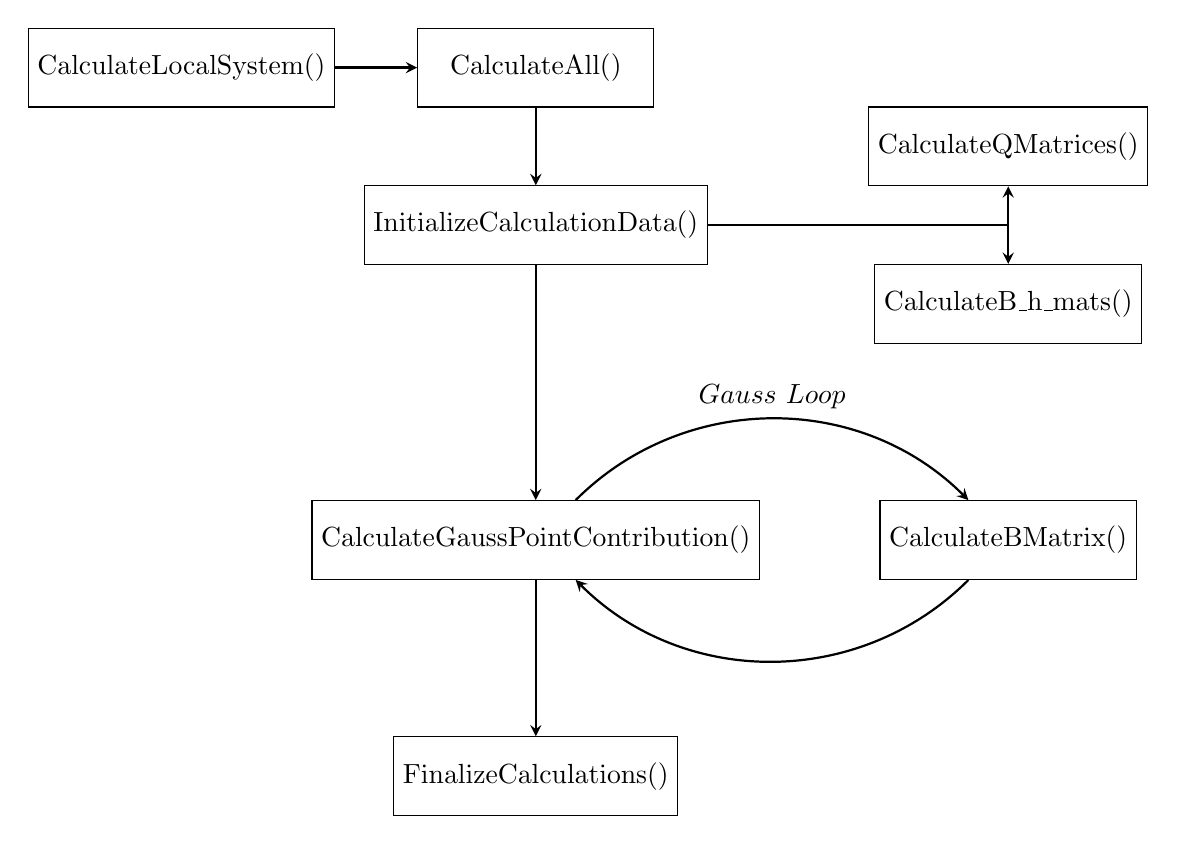
\begin{tikzpicture}[node distance = 2cm, auto]
	% Place nodes
	\node [process] (CalculateLocalSystem) {CalculateLocalSystem()};
	\node [process, right of=CalculateLocalSystem, xshift = 2.5cm] (CalculateAll) {CalculateAll()};
	\node [process, below of=CalculateAll, xshift = -0cm] (InitializeCalculationData) {InitializeCalculationData()};
	\node [process, right of=InitializeCalculationData, xshift = 4cm, yshift = 1cm] (CalculateQMatrices) {CalculateQMatrices()};
	\node [process, right of=InitializeCalculationData, xshift = 4cm, yshift = -1cm] (CalculateBhmats) {CalculateB$\_$h$\_$mats()};
	\node [process, below of=InitializeCalculationData, yshift = -2cm] (CalculateGaussPointContribution) {CalculateGaussPointContribution()};
	\node [process, right of=CalculateGaussPointContribution, xshift = 4cm] (CalculateBMatrix) {CalculateBMatrix()};
	\node [process, below of=CalculateGaussPointContribution, yshift = -1cm] (FinalizeCalculations) {FinalizeCalculations()};
	% Draw edges
	\draw [arrow] (CalculateLocalSystem) -- (CalculateAll);
	\draw [arrow] (CalculateAll) -- (InitializeCalculationData);
	\draw [arrow] (InitializeCalculationData) -| (CalculateQMatrices);
	\draw [arrow] (InitializeCalculationData) -| (CalculateBhmats);
	\draw [arrow] (InitializeCalculationData) -- (CalculateGaussPointContribution);
	\draw [arrow] (CalculateGaussPointContribution) -- (FinalizeCalculations);
	\draw [arrow] (CalculateGaussPointContribution) edge[bend left=45] node [above] {$Gauss\ Loop$} (CalculateBMatrix);
	\draw [arrow] (CalculateBMatrix) edge[bend left=45] node [below] {} (CalculateGaussPointContribution);
	\end{tikzpicture}
	\caption{High level overview of element workflow}
	\label{bendplusmemequalshell}
\end{figure}



Initially, the re-implemented purely virtual method $\texttt{CalculateLocalSystem()}$ is called by the KRATOS framework automatically for every $\texttt{ShellThinElement3D4N}$ in the job definition (.mdpa file in this case). This method simply calls $\texttt{CalculateAll()}$, which is the main pipeline of the element stiffness calculation, itself calling three key methods: $\texttt{InitializeCalculationData(),\ CalculateGaussPointContribution()}$ and $\texttt{FinalizeCalculations()}$. \\

$\texttt{InitializeCalculationData()}$ is called first, and pre-calculates quantities so they can be removed from the Gauss loop. These quantities include the basic membrane lumping matrix $\textbf{L}$, various transformation matrices ($\textbf{H}$, $\textbf{T}_{13}$, $\textbf{T}_{24}$) and all DKQ coefficients in equation  \eqref{equation23}. $\texttt{CalculateQMatrices()}$ and $\texttt{CalculateB$\_$h$\_$mats()}$ are also called from $\texttt{InitializeCalculationData()}$, which calculate $\textbf{Q}_i$ and $\textbf{B}_{hi}$ for the membrane component.\\

$\texttt{CalculateAll()}$ then calls $\texttt{CalculateGaussPointContribution()}$ which starts the Gauss integration loop. At each Gauss point $\texttt{CalculateGaussPointContribution()}$ performs Gauss integration of the expression $\textbf{K}_{contribution}$ = $\textbf{B}_{comb}^T \textbf{C} \textbf{B}_{comb}\  dA$, with the current $\textbf{B}_{comb}$ determined by calling\break$\texttt{CalculateBMatrix()}$. \\

With the Gauss integration complete, $\texttt{CalculateAll()}$ lastly calls $\texttt{FinalizeCalculations()}$ which transforms the calculated element stiffness from local to global coordinates.




























\section{Element benchmarks}

To test the correct derivation and implementation of the thin quad shell element, the shell obstacle course proposed by Belytschko \cite{Bel85} is considered.

\subsection{Scordelis-Lo roof}

The Scordelis-Lo roof is part of a cylindrical shell fixed by rigid diaphragms at it's axial ends. The only loading is a pseudo-gravity distributed load that has a magnitude of 90. Due to symmetry only a quarter of the shell is modelled. The key result is the vertical displacement of the lateral side at the midpoint, denoted by $\textcolor{red}{u}$ in the following diagram. The reference value is $u_{ref} = 0.3024$.

\begin{figure}[H]
	\centering
	\def\svgwidth{\columnwidth}
	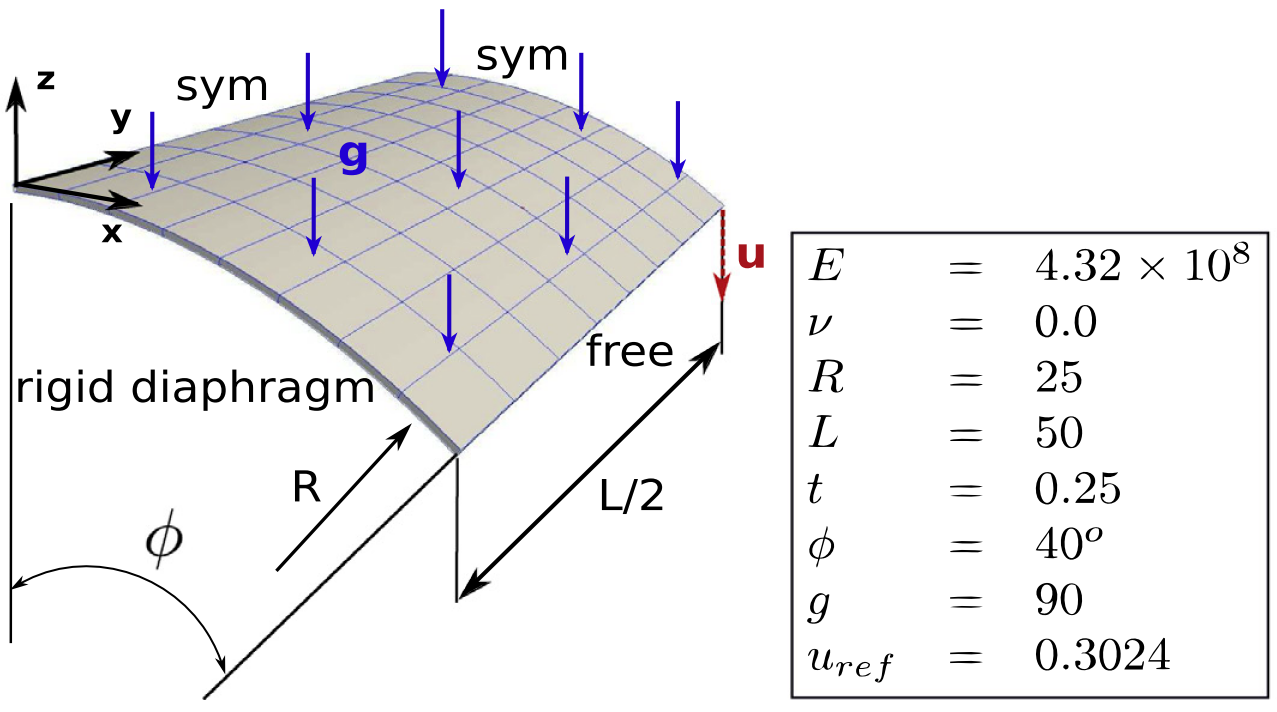
\includegraphics[width=8cm]{images/scordelisroof.png}
	\caption{Problem definition of the Scordelis-Lo roof benchmark (source: \cite{Bou13})}
	\label{scordelisroof}
\end{figure}

\pgfplotsset{width=6cm}
\begin{figure}[H]
	\centering
	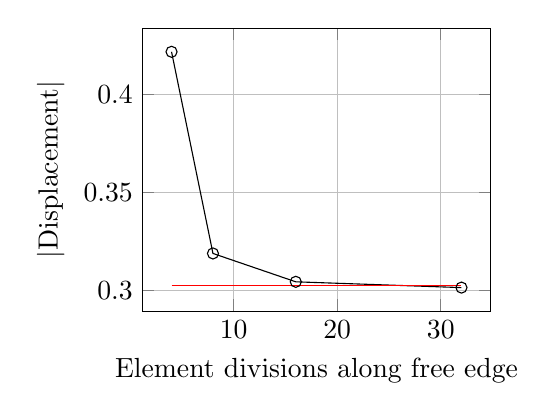
\begin{tikzpicture}
	\begin{axis}[
	xlabel=Element divisions along free edge,
	ylabel=$|$Displacement$|$,
	grid=both,]
	\addplot[color=black,mark=o] coordinates {
		(4,0.42177)
		(8,0.31887)
		(16,0.3044)
		(32,0.30145)};
	\addplot[red,domain=4:32] 
	{0.3024};
	\end{axis}
	\end{tikzpicture}
	\caption{Element convergence for the Scordelis-Lo roof benchmark}
	\label{scordelisroofbench}
\end{figure}



The performance of the element is demonstrated in the convergence graph above. It is clear that the element agrees with the reference solution.

\subsection{Pinched cylinder}

The pinched cylinder considers a cylindrical shell fixed by rigid diaphragms at it's axial ends. The loading consists of two opposing compressive point loads at the centre of the shell. Due to symmetry only an eighth of the shell is modelled. The key result is the vertical displacement under the point load, denoted by $\textcolor{red}{u}$ in the following diagram. The reference value is $u_{ref} =  1.8248\ \times\ 10^{-5}$. 

\begin{figure}[H]
	\centering
	\def\svgwidth{\columnwidth}
	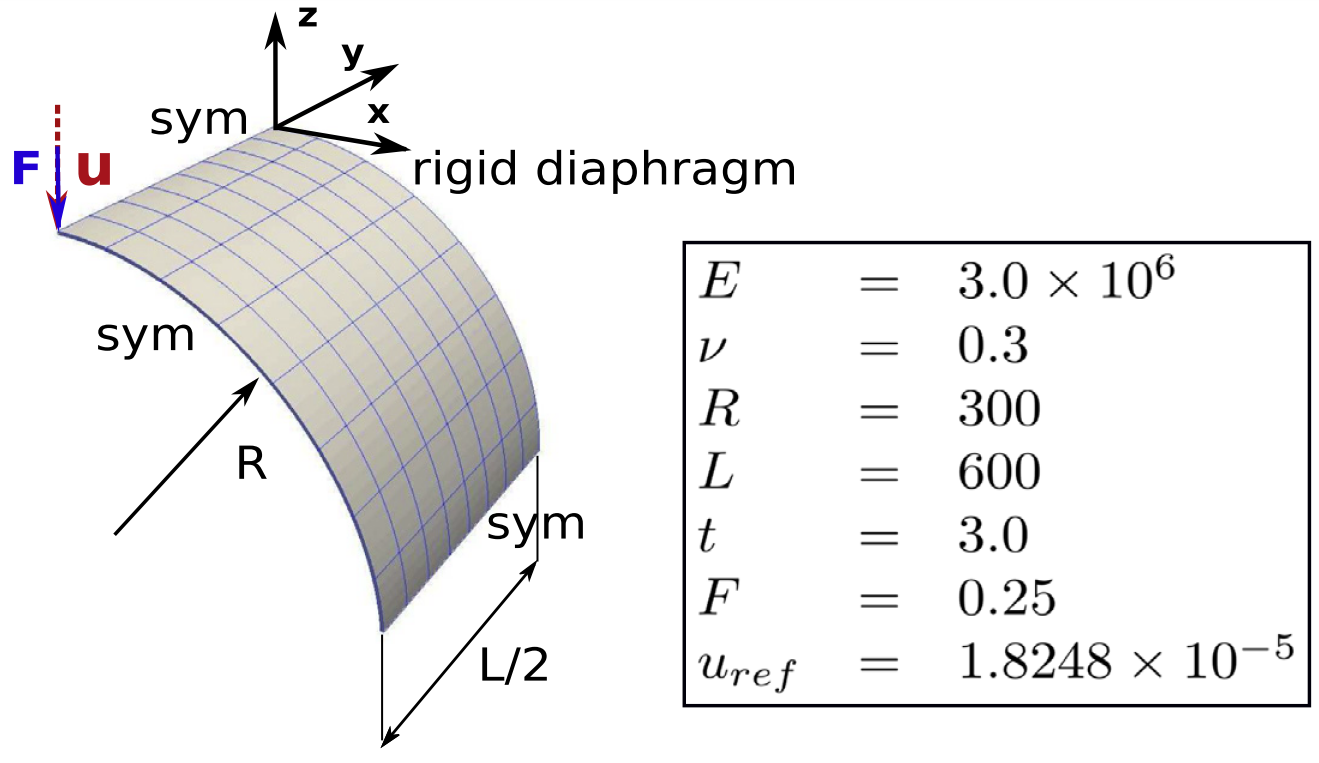
\includegraphics[width=8cm]{images/pinchedcylinder.png}
	\caption{Problem definition of the pinched cylinder benchmark (source: \cite{Bou13})}
	\label{pinchedcylinder}
\end{figure}


\pgfplotsset{width=6cm}
\begin{figure}[H]
	\centering
	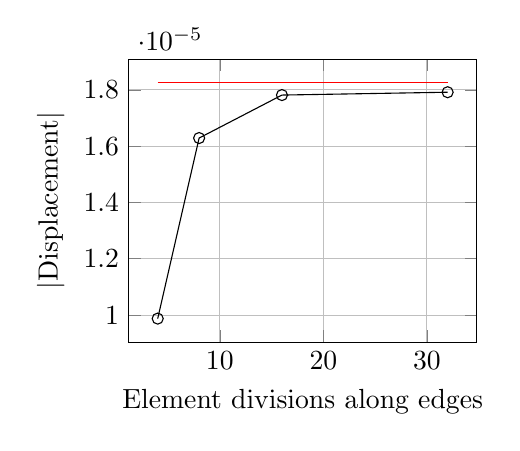
\begin{tikzpicture}
	\begin{axis}[
	xlabel=Element divisions along edges,
	ylabel=$|$Displacement$|$,
	grid=both,]
	\addplot[color=black,mark=o] coordinates {
		(4,0.0000098753)
		(8,0.0000162870)
		(16,0.0000178130)
		(32,0.0000179140)};
	\addplot[red,domain=4:32] 
	{0.000018248};
	\end{axis}
	\end{tikzpicture}
	\caption{Element convergence for the pinched cylinder benchmark}
	\label{pinchedcylinderbench}
\end{figure}



The performance of the element is demonstrated in the convergence graph above. It is clear that the element agrees with the reference solution.

\subsection{Pinched hemisphere}

The pinched hemisphere considers a hemispherical shell loaded with opposing point loads along it's equator. Due to symmetry only a quarter of the shell is modelled. The key result is the 'x' displacement along one of the point loads, denoted by $\textcolor{red}{u}$ in the following diagram. The reference value is $u_{ref} =  0.0924$. 

\begin{figure}[H]
	\centering
	\def\svgwidth{\columnwidth}
	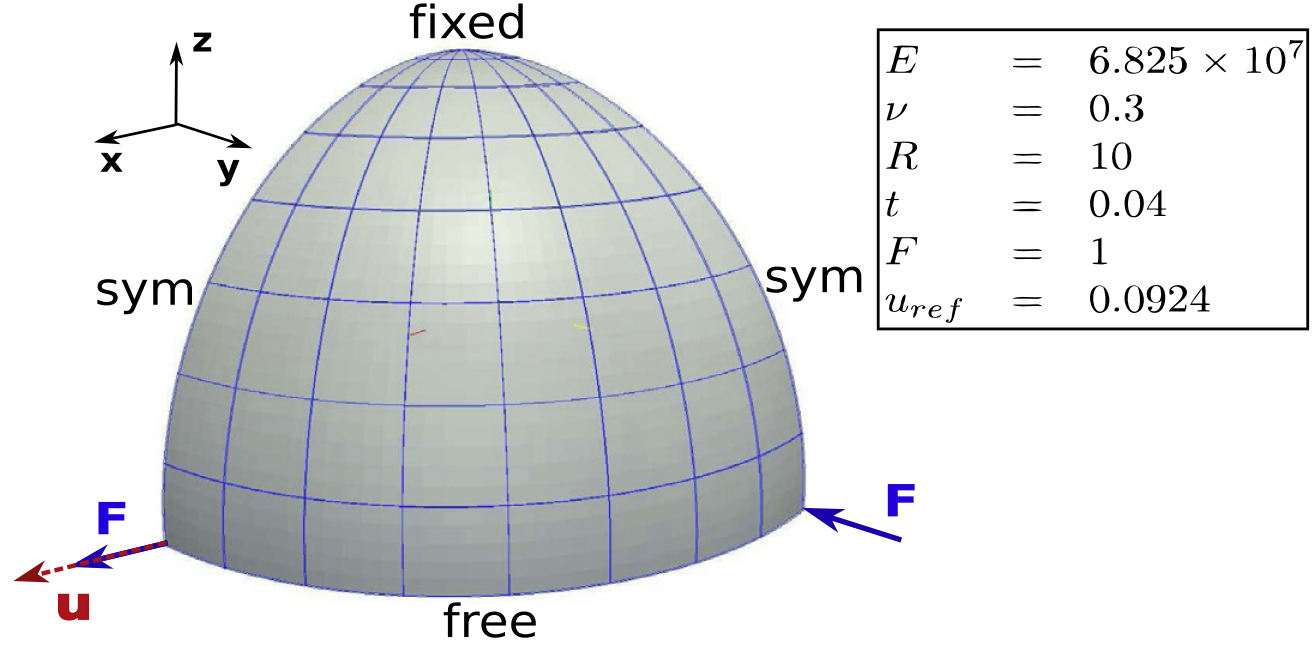
\includegraphics[width=8cm]{images/pinchedhemisphere.png}
	\caption{Problem definition of the pinched hemisphere benchmark (source: \cite{Bou13})}
	\label{pinchedhemisphere}
\end{figure}

\pgfplotsset{width=6cm}
\begin{figure}[H]
	\centering
	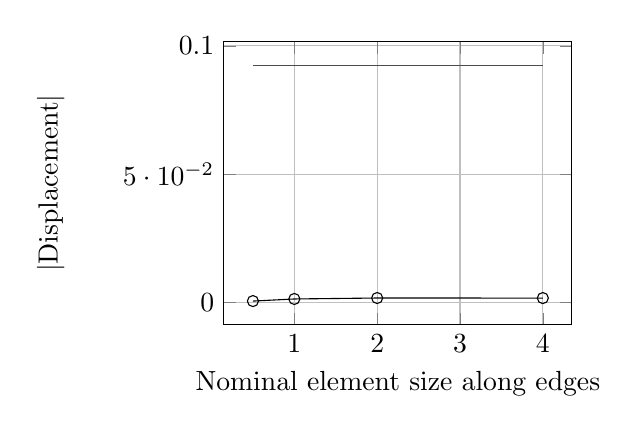
\begin{tikzpicture}
	\begin{axis}[
	xlabel=Nominal element size along edges,
	ylabel=$|$Displacement$|$,
	ylabel style={yshift=0.5cm},
	grid=both,]
	\addplot[color=black,mark=o] coordinates {
		(4,0.001648235)
		(2,0.001670075)
		(1,0.001297573)
		(0.5,0.000476183)};
	\addplot[red,domain=0.5:4] 
	{0.0924};
	\end{axis}
	\end{tikzpicture}
	\caption{Element convergence for the pinched hemisphere benchmark}
	\label{pinchedhemispherebench}
\end{figure}

Contrary to the previous benchmarks, the element does not converge to the reference solution in the pinched hemisphere test.  A key point to note is that the other benchmarks in the shell obstacle course employ a structured mesh, while the geometry of this test requires an unstructured mesh. Subsequent investigations of the element attempting to isolate remaining formulation issues have revealed the following phenomena:

\begin{itemize}
	\item Membrane tests
	\begin{itemize}
		\item[{$\times$}] Membrane tests with coarse structured meshes yield incorrect results
		\item[{$\checkmark$}] Membrane tests with fine structured meshes yield correct results
		\item[{$\times$}] Membrane tests with unstructured meshes ranging from coarse to fine yield incorrect results
	\end{itemize}
	
	\item Bending tests
	\begin{itemize}
		\item[{$\checkmark$}] Bending tests with structured meshes ranging from coarse to fine achieve correct results
		\item[{$\times$}] Bending tests with unstructured meshes ranging from coarse to fine yield incorrect results
	\end{itemize}	
\end{itemize}

From the above statements, it can be concluded that: (1) the performance of the membrane formulation is dependent on mesh refinement, and (2) the element currently handles unstructured meshes incorrectly.



















